\documentclass{snapshotmfo}

\categorizationmath{algebra and number theory,analysis,discrete mathematics and foundations,geometry and topology,numerics and scientific computing,probability theory and statistics} %at least one must be chosen. 
\categorizationconnect{chemistry and earth science,computer science,engineering and technology,finance,humanities and social sciences,life science,physics,reflections on mathematics} %can be void.
\license{CC-BY-SA-4.0} %recommended
\snapshotid{137}{1950}
\translator{german}{Trans Lator}
\junioreditor[f]{First Editor, Second Editor}{junior-editors@mfo.de}
\senioreditor[f]{Carla Cederbaum}{senior-editor@mfo.de}
\director[m]{Gerhard Huisken}

%%% Optional recommended packages
%%% Encoding
\usepackage[utf8]{inputenc}
%%% AMS mathematical facilities:
\usepackage{amsmath,amssymb}
%\usepackage{mathtools}
%%% Consistent quotation marks and citations:
%\usepackage{csquotes}

%\usepackage[ngerman]{babel}
\usepackage[spanish]{babel}
%\usepackage[USenglish]{babel}

%%% Please separate your names by \and if there are several authors.
\author{Author One\thanks{Author One is supported by the Mathematical Dreams Come True Foundation.} \and Author Two}

%%% Please insert the title of your snapshot.
\title{Spanish test file}

%%% Please provide some information on the author(s).
\authorinfo{\authorname{Author One} is a professor of pure mathematics at the First University.}
\authorinfo{\authorname{Author Two} is a lecturer in applied mathematics at the Second Institution.}

%%%%%%%%%%%%%%%% BIBLIOGRAPHY %%%%%%%%%%%%%%%%%%%%%%%%%%%%%%%%%%%%%%%%%%%%%%%%%%%%%%%%%%%%%%%%%%%%%%%%%%%%
\begin{filecontents}[overwrite]{\jobname.bib}
@book{knuth1984texbook,
  title = {The TeXbook},
  author = {Knuth, D. E.},
  year = {1984},
  edition={1},
  publisher = {Addison-Wesley}
}

@misc{wikiMath,
  author = {Wikipedia},
  title = {Mathematics --- {W}ikipedia{,} The Free Encyclopedia},
  year = {2014},
  url = {https://en.wikipedia.org/wiki/Mathematics},
  urldate = {2014-05-19}
}

@misc{sample13,
  author = {Sample, J.},
  howpublished = {\href{https://arxiv.org/abs/8765.4321v1}{arxiv:8765.4321v1}},
  title = {Interesting facts in mathematics},
  year = {2013}
}

@incollection{sample12,
  author = {Sample, J.},
  title = {Things you don't know about mathematics},
  booktitle = {A bookseries about mathematics},
  publisher = {Some publisher},
  year = {2012}
}

@inproceedings{sample11,
  author={Example, C.},
  title={A new perspective on mathematics},
  booktitle={New perspectives on arts and sciences},
  year={2011}
}

@phdthesis{sample14,
  author={Candidate, A.},
  title={Thesis title},
  school={MFO},
  year={2014}
}
\end{filecontents}
%%%%%%%%%%%%%%%%%%%%%%%%%%%%%%%%%%%%%%%%%%%%%%%%%%%%%%%%%%%%%%%%%%%%%%%%%%%%%%%%%%%%%%%%%%%%%%%%%%%%%%%%%%

\begin{document}

\begin{abstract}
Does this snapshot using the spanish option of the babel package compile? Are the automatically generated snippets all spanish?
\end{abstract}

\section{Autoref} \label{sec:autoref}
The hyperref package handles various types of labels enumerated independently of each other, e.\,g.
for figures, tables, equations, sections, subsections, and subsubsections.
\verb+\autoref{<labelname>}+ returns the labels together with their respective types {\em in the chosen language}.

\subsection{References}
The references are given first to make them appear on the first page:
\begin{itemize}
\item[] The Mayan figure is referenced as \autoref{fig:maya}.
\item[] The test table is referenced as \autoref{tab:dull}.
\item[] The classical equation is referenced as \autoref{eq:pythagoras}.
\item[] The theorem is referenced as \autoref{thm:continuity}.
\item[] The ``autoref'' section is referenced as \autoref{sec:autoref}.
\item[] The ``labels'' subsection is referenced as \autoref{subsec:labels}.
\item[] The sample subsubsection is referenced as \autoref{subsubsec:sample}.
\item[] The page of the Mayan figure is referenced as \autopageref{fig:maya}.
\end{itemize}

\subsection{Labels} \label{subsec:labels}
The labeled objects missing so far are defined in this subsection.

% sample figure
\begin{figure}[ht]
  \centering 
  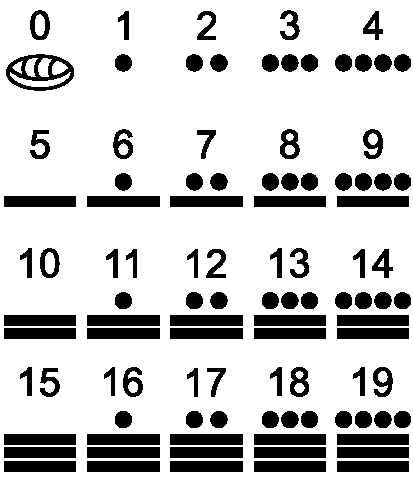
\includegraphics[width= 0.33 \textwidth]{maya.pdf}
  \caption{Exemplary image: Maya numerals.}
  \label{fig:maya}
\end{figure}

% sample table
\begin{table}[ht]
  \caption{test table}
  \begin{tabular}{ l c r }
    1 & 2 & 3 \\
    4 & 5 & 6 \\
    7 & 8 & 9 \\
  \end{tabular}
  \label{tab:dull}
\end{table}

\subsubsection{Sample subsubsection} \label{subsubsec:sample}

% sample equation
\begin{equation}\label{eq:pythagoras}
a^2+b^2=c^2
\end{equation}

% sample theorem
\newtheorem{theorem}{Theorem}
\begin{theorem}\label{thm:continuity}
Let $f$ be a function whose derivative exists in every point, then $f$ 
is a continuous function.
\end{theorem}

As usual, you can give references such as \cite{knuth1984texbook, wikiMath, sample13, sample12, sample11, sample14} via the \verb+\cite+ command.

\begin{imagecredits}
  \item[\autoref{fig:maya}] ``Maya''. Author: Bryan Derkson. Licensed under Creative Commons Attribution-Share Alike 3.0 via Wikimedia Commons, \url{https://commons.wikimedia.org/wiki/File:Maya.svg}, visited on \printdate{2014-09-05}.
\end{imagecredits}

\clearpage

\bibliography{\jobname}
\end{document}
